\section{Results}\label{chap6:Results}

The \mti{} distributions for the signal region after the full analysis selection
are shown in Fig.~\ref{fig:13TeVmTishapes} for the three jet categories.
 Two different signal hypotheses corresponding to $M_\mathrm{X} = 400$\GeV and
 $M_\mathrm{X} = 800$\GeV are shown superimposed on the background for comparison.

\begin{figure}[!htb]
\centering
\subfigure[0 jets]{
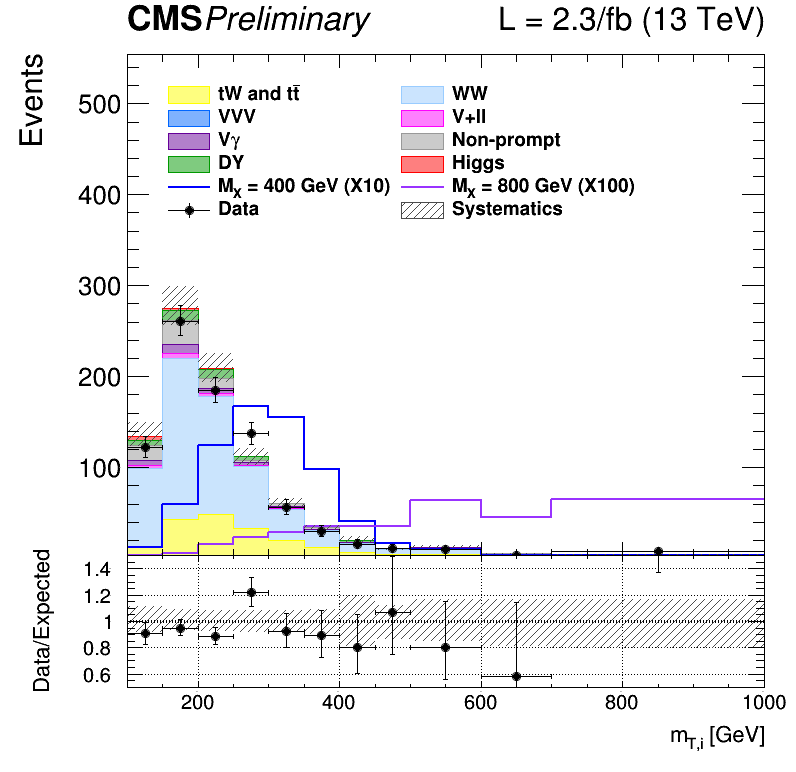
\includegraphics[width=0.45\textwidth]{images/13TeV/HighMass/cratio_hwwhm_13TeV_of_0j_mTi.png}
}
\subfigure[1 jet]{
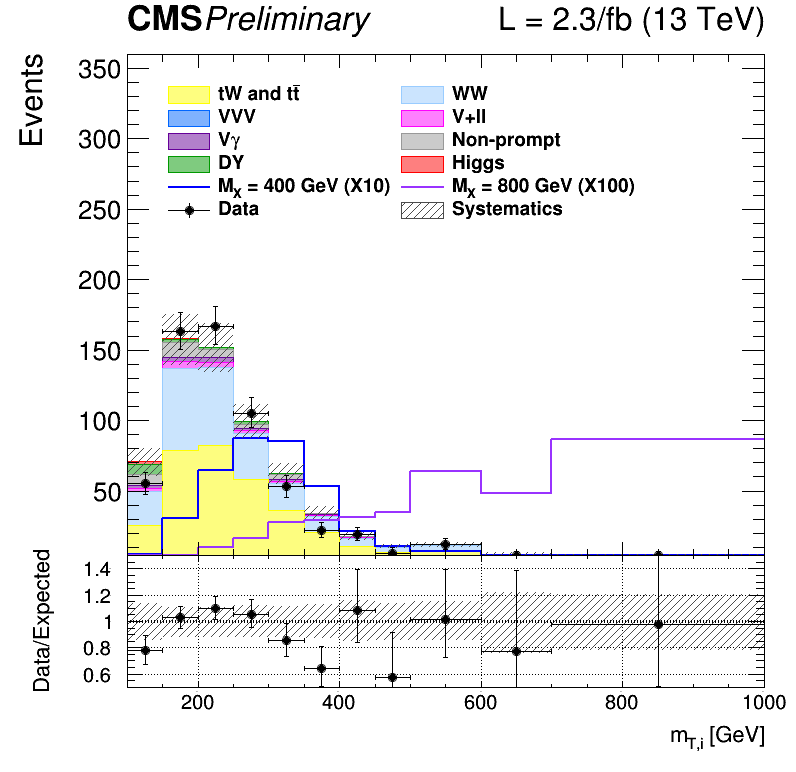
\includegraphics[width=0.45\textwidth]{images/13TeV/HighMass/cratio_hwwhm_13TeV_of_1j_mTi.png}
}
\\
\subfigure[VBF]{
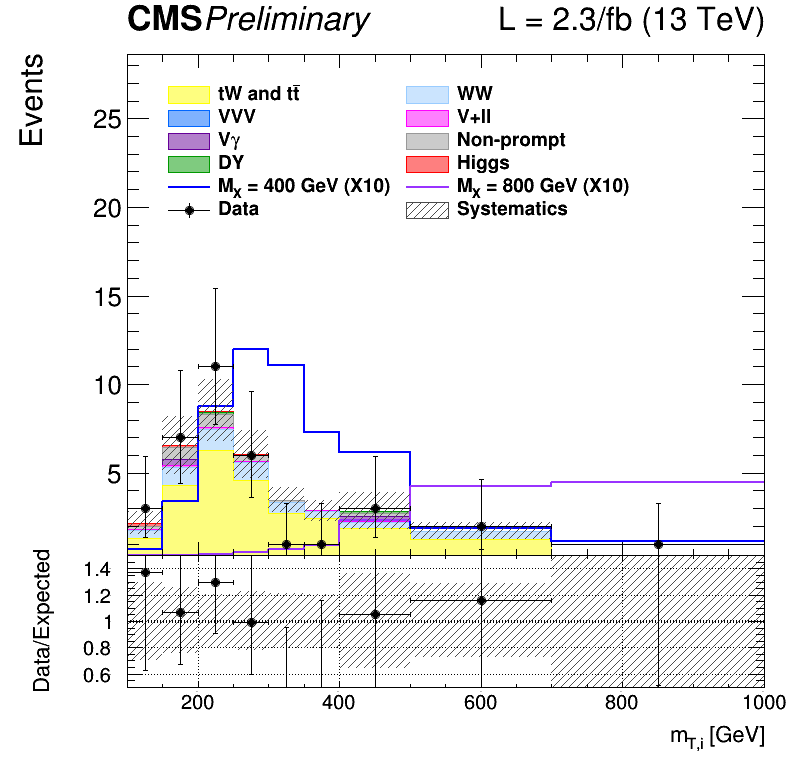
\includegraphics[width=0.45\textwidth]{images/13TeV/HighMass/cratio_hwwhm_13TeV_of_VBF_mTi_VBF.png}
}
\caption{
    Distributions of \mti{} in the signal region for the 0 jets, 1 jet and VBF categories. Background normalization corresponds to the pre-fit value. Signal contributions for two mass hypotheses, $M_\mathrm{X} = 400$\GeV and $M_\mathrm{X} = 800$\GeV, are shown superimposed on the background and scaled to facilitate the comparison.}
    \label{fig:13TeVmTishapes}
\end{figure}

For every mass point from 200\GeV up to 1\TeV the observed p-value and the 95\% CL upper exclusion limit are calculated for four hypotheses of the signal decay width. The observed p-value as a function of the resonance mass for the combination of the three jet categories is shown in Table~\ref{tab:significance}.

\begin{table}[htb]
\small{
\begin{center}
\caption{Observed p-value and corresponding significance (set to 0 in case of underfluctuations of the observed number of events) for the combination of the three jet categories for different resonance masses. Different values of the signal width are shown.\label{tab:significance}}
\begin{tabular}{lcccccc}
\toprule
\multirow{2}{*}{Mass [GeV]}            & $\Gamma = 0.09 \times \Gamma_{SM}$ & $\Gamma = 0.25 \times \Gamma_{SM}$ & $\Gamma = 0.49 \times \Gamma_{SM}$ & $\Gamma = \Gamma_{SM}$\\
                                          & p-value (signif.)  & p-value (signif.)  & p-value (signif.)  & p-value (signif.) \\
\midrule
200 &  0.50 (0)   & 0.50 (0)    & 0.50 (0) & 0.56 (0)\\
210 &  0.58 (0)   & 0.45 (0.1) & 0.35 (0.4) & 0.24 (0.7)\\
230 &  0.21 (0.8) & 0.22 (0.8) & 0.23 (0.7) & 0.26 (0.6)\\
250 &  0.29 (0.5) & 0.20 (0.8)  & 0.15 (1.0) & 0.12 (1.2)\\
300 &  0.014 (2.2)& 0.015 (2.2)& 0.016 (2.1) & 0.018 (2.1)\\
350 &  0.16 (1.0) & 0.17 (1.0) & 0.18 (0.9) & 0.23 (0.7)\\
400 &  0.50 (0)   & 0.49 (0)   & 0.49 (0) & 0.57 (0)\\
450 &  0.51 (0)   & 0.50 (0)   & 0.50 (0) & 0.52 (0)\\
500 &  0.50 (0)   & 0.51 (0)   & 0.50 (0) & 0.52 (0)\\
550 &  0.50 (0)   & 0.51 (0)   & 0.51 (0) & 0.51 (0)\\
600 &  0.50 (0)   & 0.50 (0)   & 0.51 (0) & 0.51 (0)\\
650 &  0.50 (0)   & 0.50 (0)   & 0.54 (0) & 0.50 (0)\\
700 &  0.50 (0)   & 0.50 (0)   & 0.50 (0) & 0.50 (0)\\
750 &  0.50 (0)   & 0.54 (0)   & 0.50 (0) & 0.40 (0.3)\\
800 &  0.50 (0)   & 0.55 (0)   & 0.39 (0.3) & 0.29 (0.6)\\
900 &  0.29 (0.6) & 0.27 (0.6) & 0.24 (0.7) & 0.22 (0.8)\\
1000 & 0.18 (0.9) & 0.18 (0.9) & 0.18 (0.9) & 0.18 (0.9)\\
\bottomrule
\end{tabular}
\end{center}
}
\end{table}

In order to be independent on the particular model assumed for the signal cross section, the results are interpreted as exclusion limits on $\sigma \times \mathcal{B}$, where $\sigma$ stands for the sum of the ggH and VBF cross sections, and $\mathcal{B}$ represents the $\mathrm{X\to WW \to2\ell2\nu}$ branching ratio including all lepton flavours. The expected and observed upper exclusion limits on $\sigma \times \mathcal{B}$ for $\Gamma' = \Gamma_\mathrm{SM}$ are shown in Fig.~\ref{fig:13TeVobslim}.

\begin{figure}[htb]
\centering
\subfigure[0 jets]{
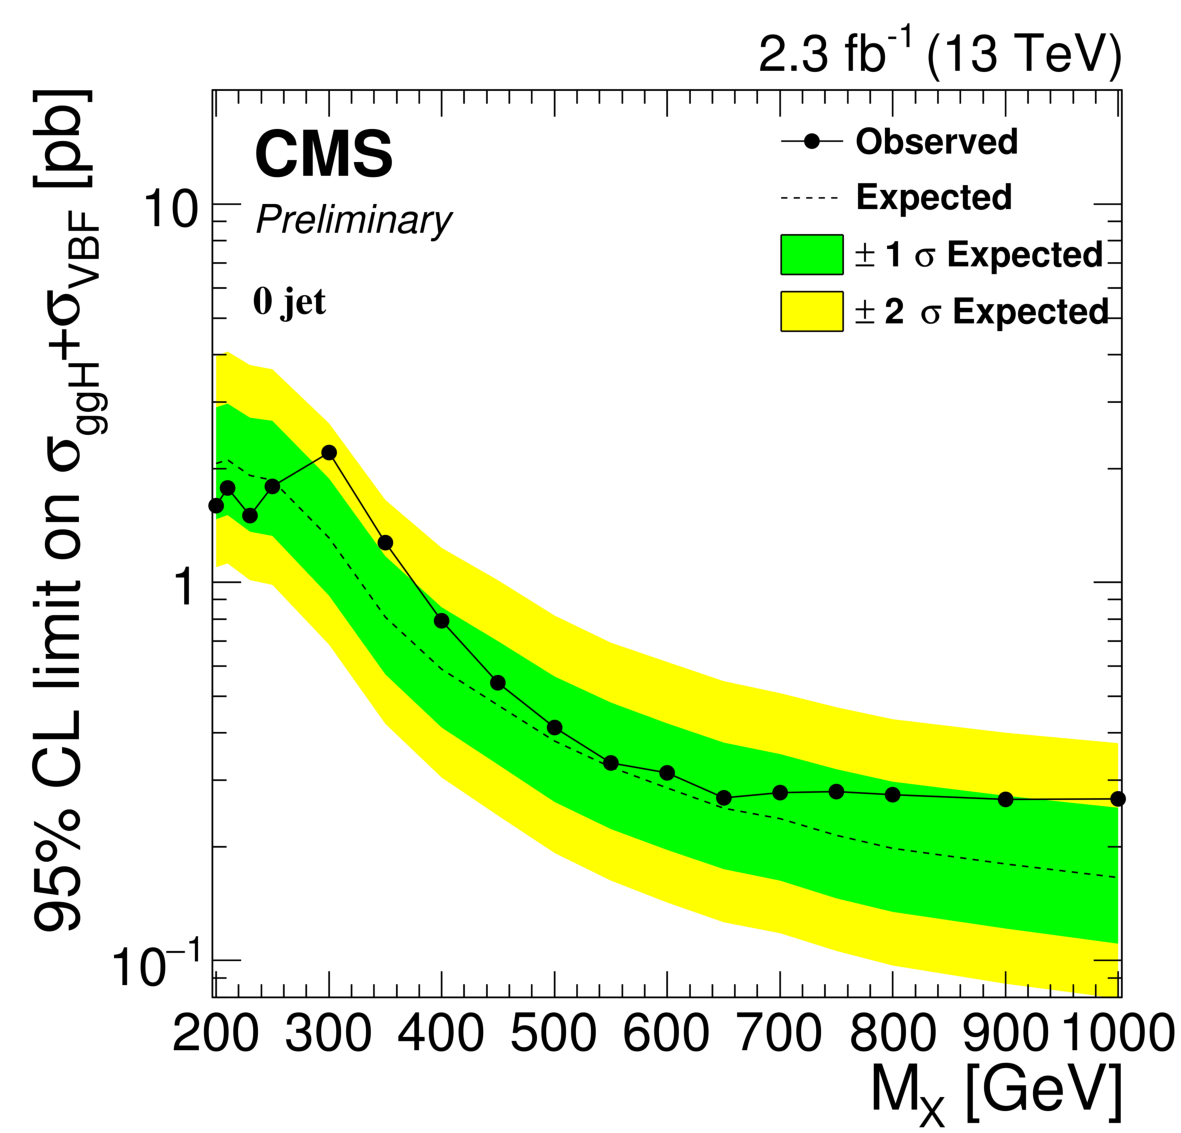
\includegraphics[width=0.45\textwidth]{images/13TeV/HighMass/obs_limit_0jet_xsec.pdf}
}
\subfigure[1 jet]{
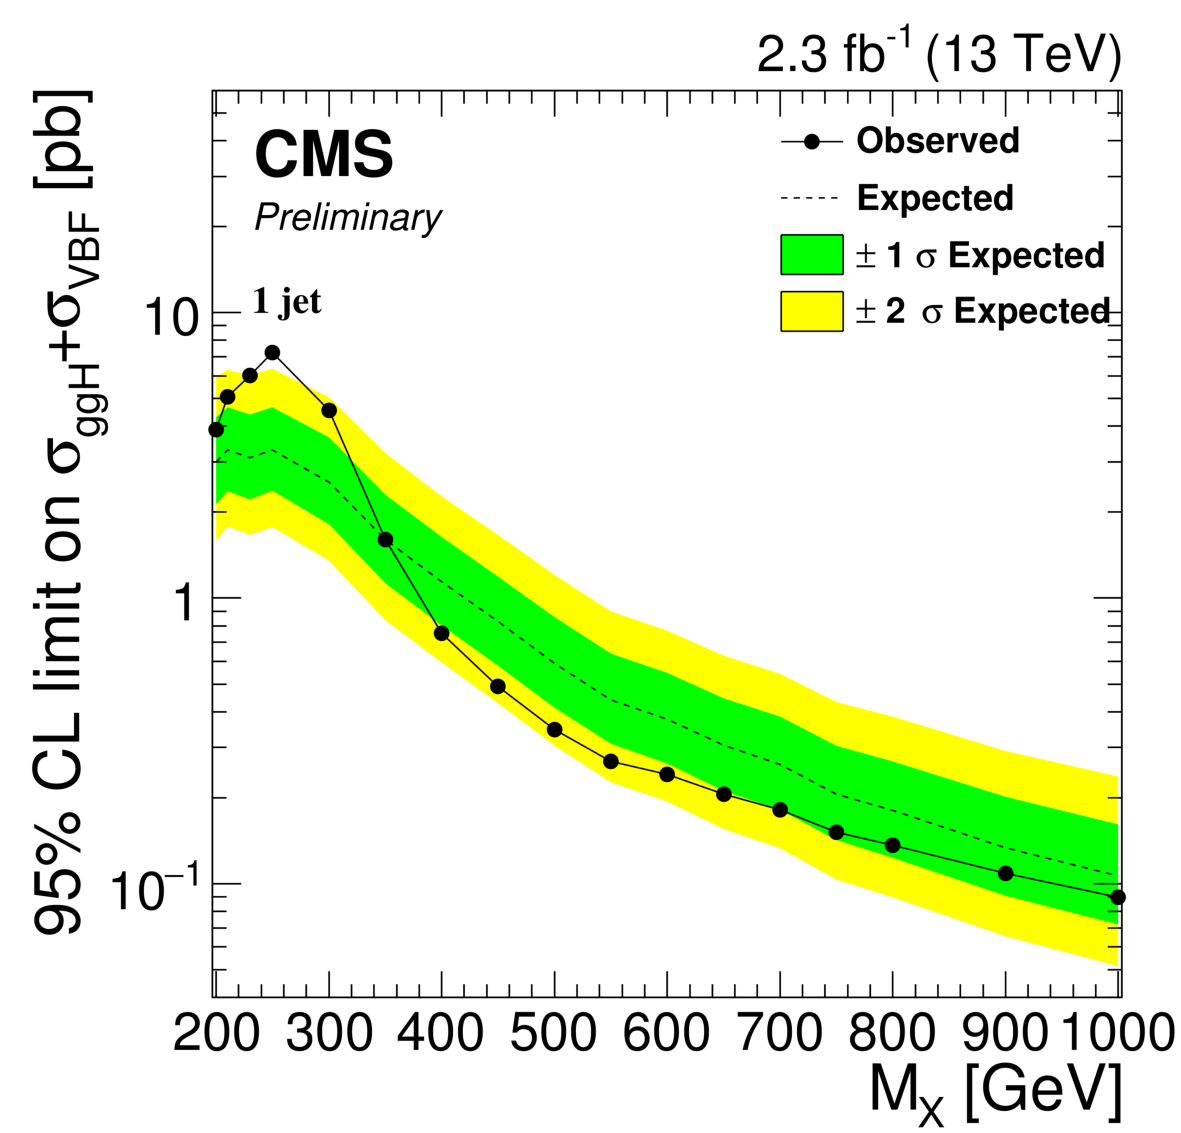
\includegraphics[width=0.45\textwidth]{images/13TeV/HighMass/obs_limit_1jet_xsec.pdf}
}\\
\subfigure[VBF]{
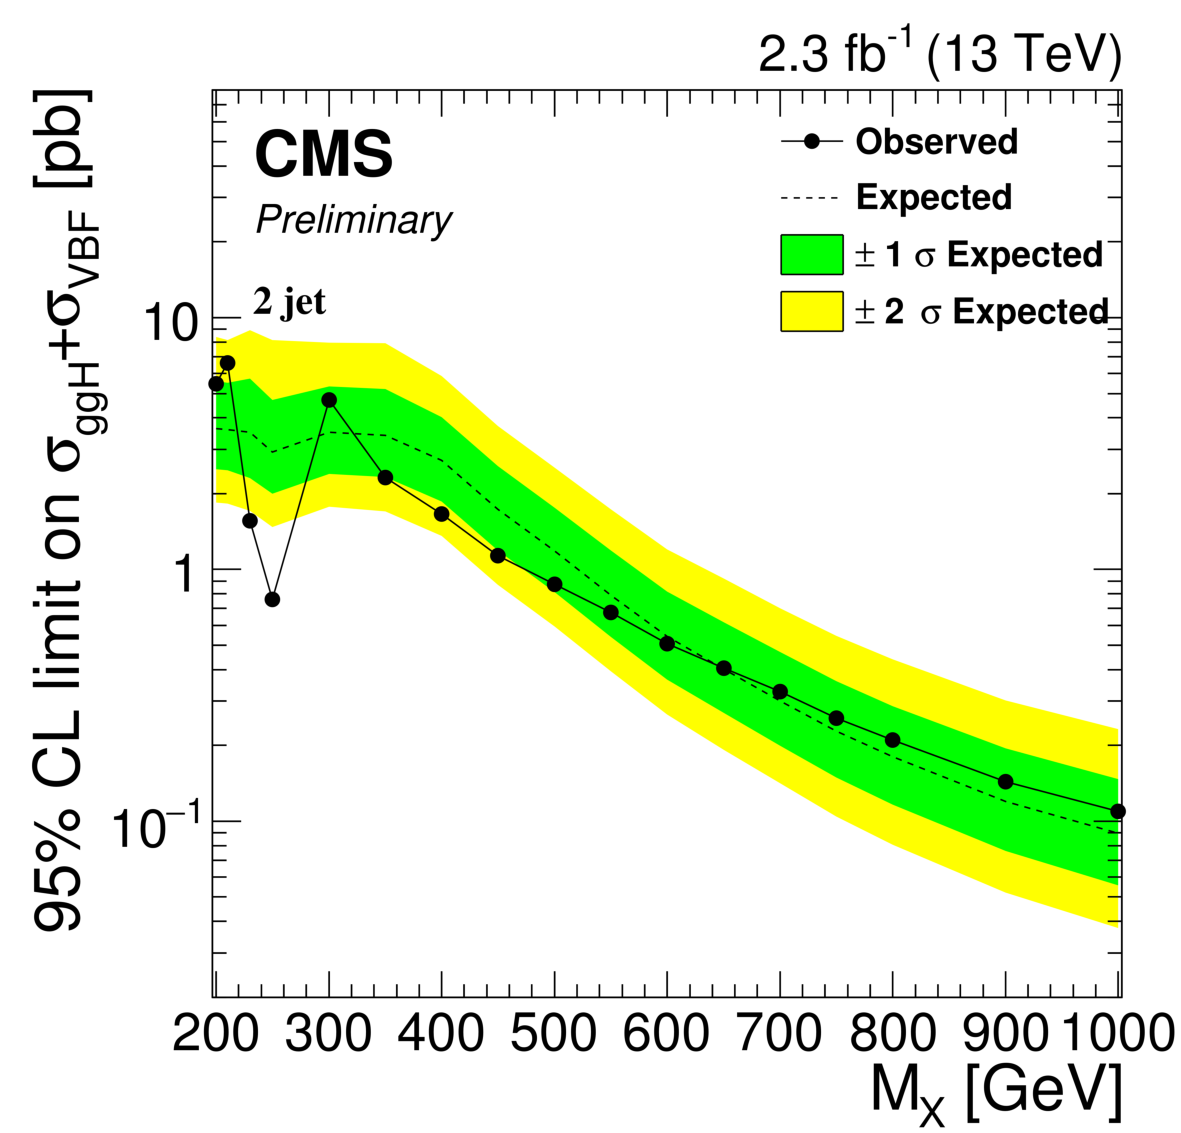
\includegraphics[width=0.45\textwidth]{images/13TeV/HighMass/obs_limit_2jet_xsec.pdf}
}
\caption{Expected and observed exclusion upper limits at 95\% CL on $\sigma \times \mathcal{B}$ in the three categories, as a function of the resonance mass. The dashed line corresponds to the median upper limit, while the green and yellow regions represent the $\pm 1\sigma$ and $\pm 2 \sigma$ uncertainty bands, respectively. The dotted line represents the observed limit. Limits are derived assuming $\Gamma' = \Gamma_\mathrm{SM}$ for each mass point.}\label{fig:13TeVobslim}
\end{figure}

A mild excess is observed in the 0 jets category and, more evident, in the 1 jet category around 250--300\GeV. A deficit is instead observed in the VBF category around 250\GeV, which is mainly due to an underfluctuation of the background. This effect can be understood looking at the VBF shape in Fig.~\ref{fig:13TeVmTishapes}, where two adjacent data points, corresponding to the fifth and sixth bins of the \mti distribution, clearly underfluctuate with respect to the background prediction, causing the dip in the observed limit.

The exclusion limit resulting from the combination of the three categories is shown in Fig.~\ref{fig:13TeVcombobslim}, for the four $\Gamma'$ hypotheses discussed before. From the combined exclusion limits no significant evidence of a deviation from the background only hypothesis is observed. In the case the new resonance has the same decay width as the SM Higgs boson, i.e. $\Gamma'=\Gamma_\mathrm{SM}$, the expected cross section times branching ratio is also displayed, excluding this hypothesis in the mass range from 350 to 550\GeV.
%The presence of a scalar resonance with $\sigma\times\mathcal{B}$ higher than the values reported in Fig.~\ref{fig:13TeVcombobslim} is thus excluded with a 95\% CL for masses ranging from 200\GeV up to 1\TeV. 

\begin{figure}[htb]
\centering
\subfigure{
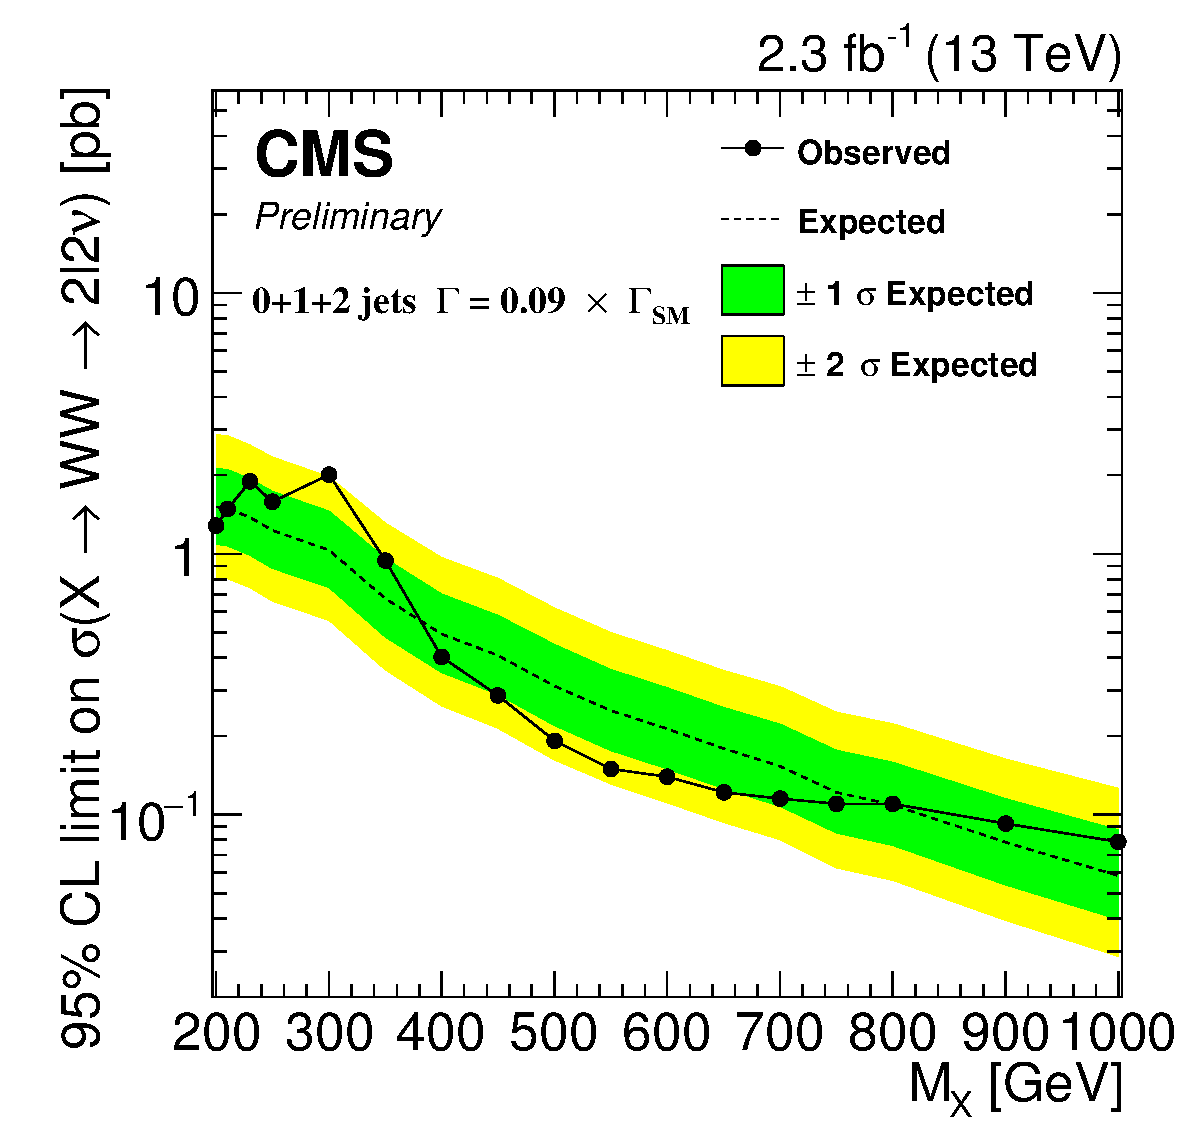
\includegraphics[width=0.45\textwidth]{images/13TeV/HighMass/limit_009GSM_PAS.pdf}
}
\subfigure{
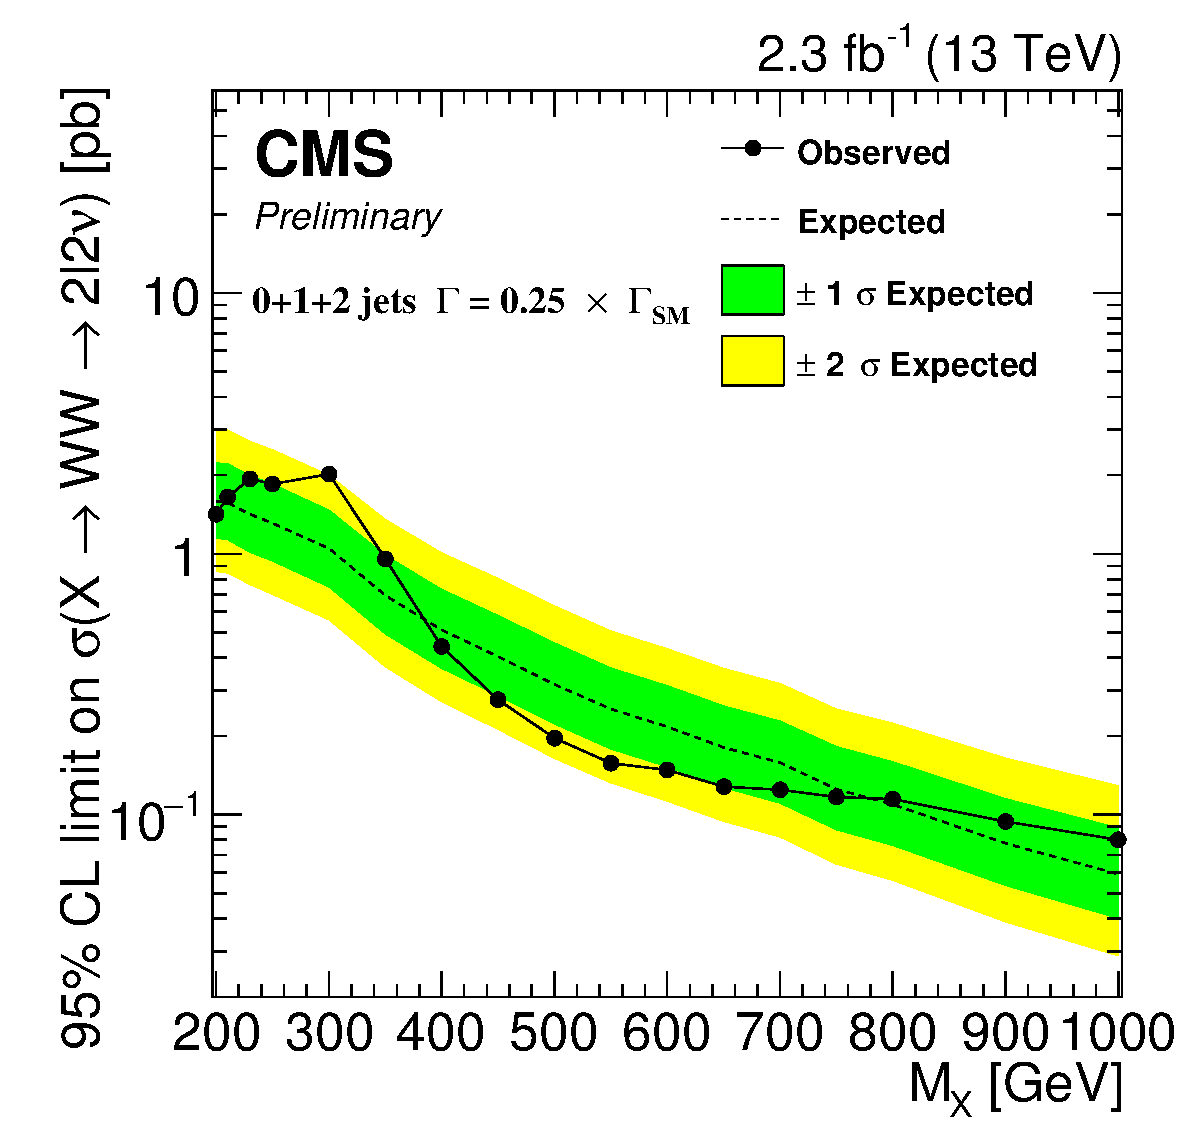
\includegraphics[width=0.45\textwidth]{images/13TeV/HighMass/limit_025GSM_PAS.pdf}
}
\\
\subfigure{
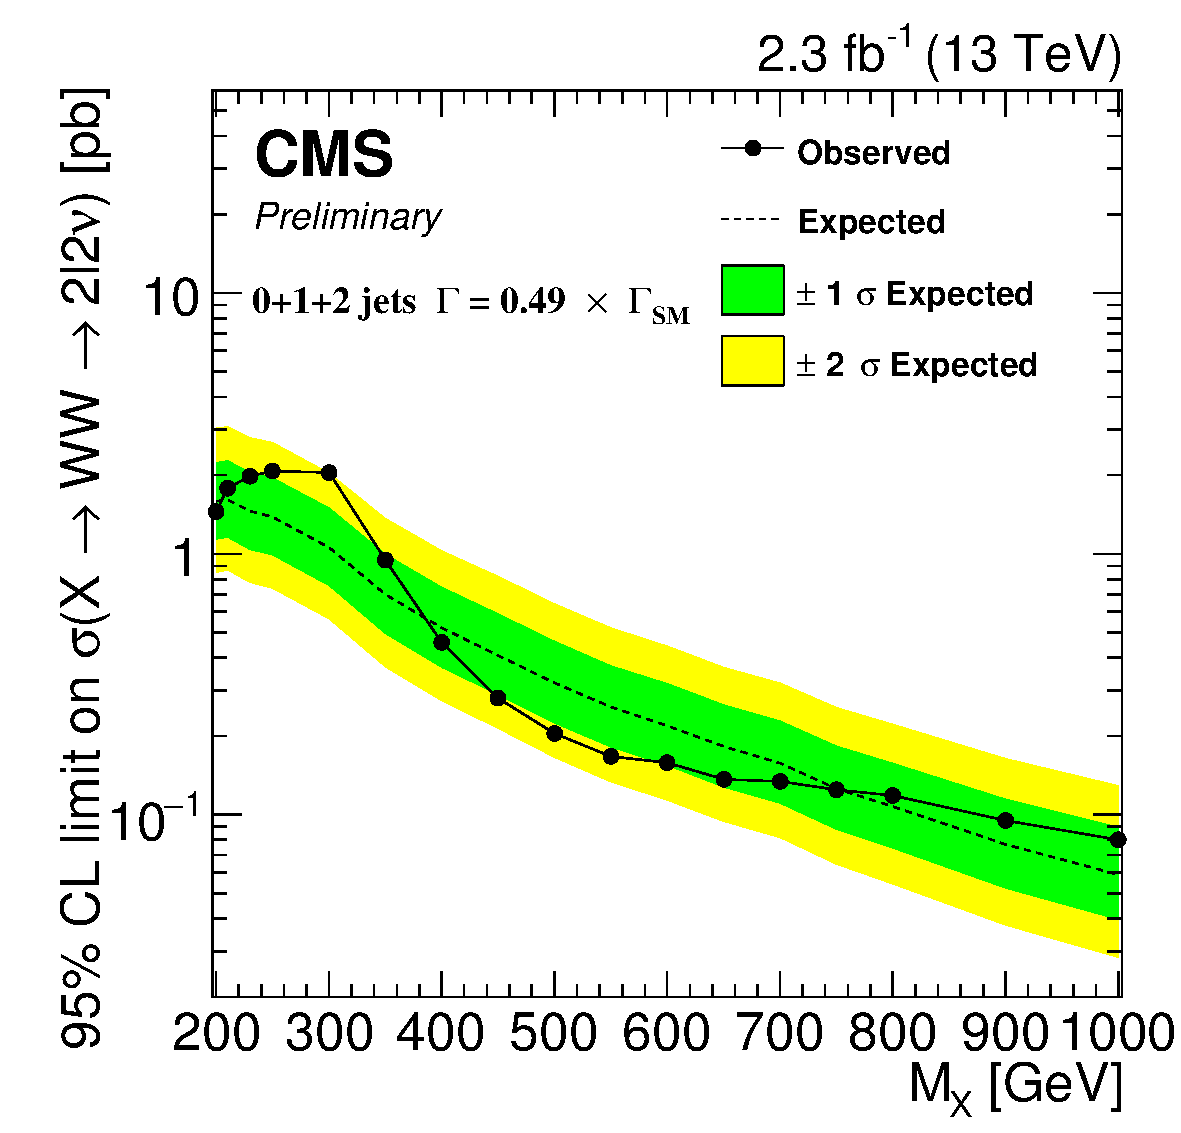
\includegraphics[width=0.45\textwidth]{images/13TeV/HighMass/limit_049GSM_PAS.pdf}
}
\subfigure{
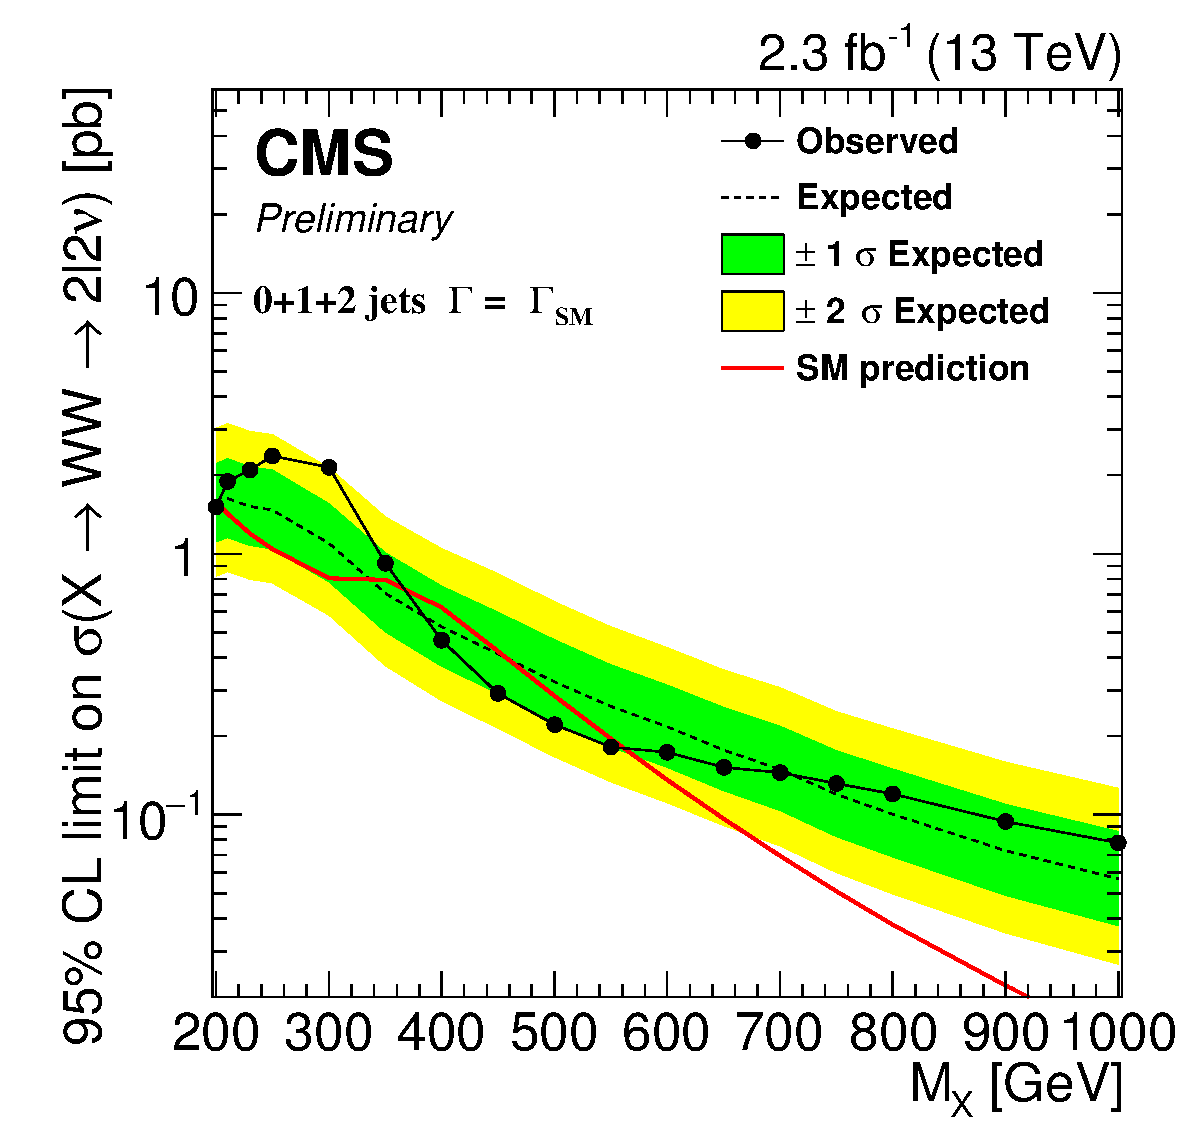
\includegraphics[width=0.45\textwidth]{images/13TeV/HighMass/limit_GSM_SMprediction.pdf}
}
\caption{
    Expected and observed exclusion limits at 95\% CL on $\sigma\times\mathcal{B}$ for the combination of the three jet categories as a function of the resonance mass. The black dotted line corresponds to the observed value while the yellow and green bands represent the $\pm 1 \sigma$ and $\pm 2 \sigma$ uncertainties respectively. Limits are displayed for four decay width hypotheses. In the case of $\Gamma' = \Gamma_{\rm SM}$ the cross section prediction is displayed as a red line.}
    \label{fig:13TeVcombobslim}
\end{figure}

